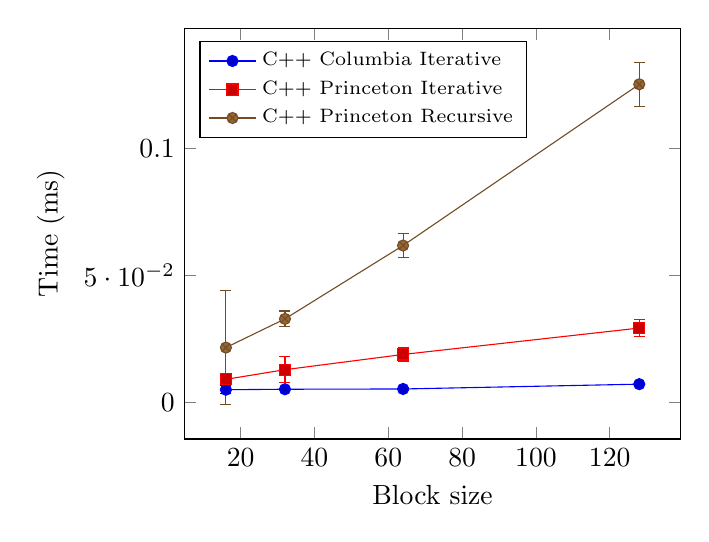
\begin{tikzpicture}
\begin{axis}[xlabel={Block size},ylabel={Time (ms)},width=0.65\linewidth,legend pos=north west,scaled y ticks = false,legend cell align=left,legend style={font=\scriptsize}]
\addplot+[error bars/.cd, y dir=both,y explicit] coordinates {
(16, 0.0049) +- (0.0015, 0.0015)
(32, 0.0051) +- (0.0002, 0.0002)
(64, 0.0052) +- (0.0005, 0.0005)
(128, 0.0071) +- (0.0003, 0.0003)
};
\addplot+[error bars/.cd, y dir=both,y explicit] coordinates {
(16, 0.0090) +- (0.0022, 0.0022)
(32, 0.0128) +- (0.0052, 0.0052)
(64, 0.0188) +- (0.0029, 0.0029)
(128, 0.0292) +- (0.0032, 0.0032)
};
\addplot+[error bars/.cd, y dir=both,y explicit] coordinates {
(16, 0.0215) +- (0.0225, 0.0225)
(32, 0.0328) +- (0.0031, 0.0031)
(64, 0.0617) +- (0.0047, 0.0047)
(128, 0.1252) +- (0.0086, 0.0086)
};
\legend{C++ Columbia Iterative , C++ Princeton Iterative , C++ Princeton Recursive}
\end{axis}
\end{tikzpicture}
